% Transformer Block Detail
% Compile with: pdflatex transformer_block.tex
%
\documentclass[border=8pt]{standalone}
\usepackage[T1]{fontenc}
\usepackage{tikz}
\usepackage{amsmath,amssymb}
\usetikzlibrary{
    arrows.meta,
    positioning,
    calc,
    fit,
    backgrounds
}

% ── Color Palette ──
\definecolor{blockcol}{HTML}{EF9A9A}
\definecolor{normcol}{HTML}{C5E1A5}
\definecolor{attncol}{HTML}{FFAB91}
\definecolor{mlpcol}{HTML}{90CAF9}
\definecolor{framecol}{HTML}{757575}

\begin{document}
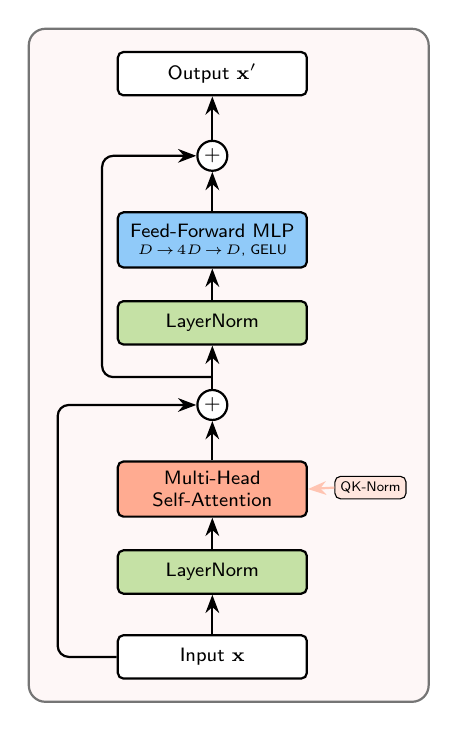
\begin{tikzpicture}[
    >=Stealth,
    font=\sffamily\footnotesize,
    smod/.style={
        draw, thick, rounded corners=2pt,
        minimum width=2.4cm, minimum height=0.55cm,
        align=center, font=\sffamily\scriptsize
    },
    addcirc/.style={
        draw, thick, circle, inner sep=0pt,
        minimum size=0.38cm, fill=white,
        font=\sffamily\scriptsize\bfseries
    },
    arr/.style={->, >=Stealth, thick},
]

% ── Nodes (bottom to top) ──

% Input
\node[smod, fill=white] (bin) at (0, 1.5) {Input $\mathbf{x}$};

% --- First sub-block: LN + MHSA ---
\node[smod, fill=normcol, above=0.50cm of bin] (bln1) {LayerNorm};

\node[smod, fill=attncol, minimum height=0.7cm, above=0.40cm of bln1] (bmha) {
    Multi-Head\\Self-Attention
};

% QK-Norm annotation
\node[draw, rounded corners=2pt, fill=attncol!30,
      font=\sffamily\tiny, inner sep=2pt,
      anchor=west] (qknorm) at (1.55, 3.65) {QK-Norm};
\draw[thick, attncol!70, ->] (qknorm.west) -- (bmha.east);

% Add node 1
\node[addcirc, above=0.50cm of bmha] (badd1) {$+$};

% --- Second sub-block: LN + MLP ---
\node[smod, fill=normcol, above=0.55cm of badd1] (bln2) {LayerNorm};

\node[smod, fill=mlpcol, minimum height=0.7cm, above=0.40cm of bln2] (bmlp) {
    Feed-Forward MLP\\[-2pt]
    {\tiny $D \!\to\! 4D \!\to\! D$, GELU}
};

% Add node 2
\node[addcirc, above=0.50cm of bmlp] (badd2) {$+$};

% Output
\node[smod, fill=white, above=0.55cm of badd2] (bout) {Output $\mathbf{x}'$};

% ── Main flow arrows ──
\draw[arr] (bin) -- (bln1);
\draw[arr] (bln1) -- (bmha);
\draw[arr] (bmha) -- (badd1);
\draw[arr] (badd1) -- (bln2);
\draw[arr] (bln2) -- (bmlp);
\draw[arr] (bmlp) -- (badd2);
\draw[arr] (badd2) -- (bout);

% ── Residual Connections (black, left side, rounded corners) ──
% Residual 1: Input → Add1 (bypasses LN1 + MHSA)
\draw[arr, rounded corners=4pt]
    (bin.west) -- ++(-0.75, 0) |- (badd1.west);

% Residual 2: after Add1 → Add2 (bypasses LN2 + MLP)
\coordinate (r2fork) at ($(badd1.north) + (0, 0.15)$);
\draw[arr, rounded corners=4pt]
    (r2fork) -- ++(-1.4, 0) |- (badd2.west);

% Helper coordinate for residual left extent
\coordinate (res_left) at (-2.05, 4.6);

% Background frame — fit to content
\begin{scope}[on background layer]
    \node[draw, thick, rounded corners=6pt,
          color=framecol, fill=blockcol!8,
          inner sep=8pt,
          fit=(bin)(bout)(qknorm)(res_left)]
          (bframe) {};
\end{scope}

\end{tikzpicture}
\end{document}
